\documentclass{sig-alternate-2013}
\permission{Copyright is held by the International World Wide Web Conference Committee (IW3C2). IW3C2 reserves the right to provide a hyperlink to the author's site if the Material is used in electronic media.}
\conferenceinfo{WWW'14 Companion,}{April 7--11, 2014, Seoul, Korea.} 
\copyrightetc{ACM \the\acmcopyr}
\crdata{978-1-4503-2744-2/14/04. \\ http://dx.doi.org/10.1145/2567948.2576960}

\clubpenalty=10000 
\widowpenalty = 10000


\usepackage{eurosym}
\usepackage{url}
\usepackage{hyperref}
\usepackage[tracking=true]{microtype}

\begin{document}

\title{Crowd vs. Experts: Nichesourcing for Knowledge Intensive Tasks in Cultural Heritage}

\numberofauthors{3}
\author{
% 1st. author
\alignauthor 
Jasper Oosterman, \\Alessandro Bozzon, Geert-Jan Houben \\
       \affaddr{Delft University of Technology} \\
       \affaddr{Delft, The Netherlands} \\
       \email{j.e.g.oosterman, a.bozzon, g.j.p.m.houben@tudelft.nl}
\and
% 2nd. author
\alignauthor Archana Nottamkandath, 	\\Chris Dijkshoorn, Lora Aroyo \\
       \affaddr{VU University Amsterdam} \\
       \affaddr{Amsterdam, The Netherlands} \\
       \email{a.nottamkandath, c.r.dijkshoorn, lora.aroyo@vu.nl}
% 3rd. author
\and  % use '\and' if you need 'another row' of author names
% 4th. author
\alignauthor  Mieke~H.~R.~Leyssen, Myriam~C.~Traub \\
       \affaddr{Centrum Wiskunde \& Informatica}\\
       \affaddr{Amsterdam, The Netherlands}\\
       \email{mieke.leyssen, myriam.traub@cwi.nl}
       }

\maketitle   
       
\begin{abstract}
The results of our exploratory study provide new insights to crowdsourcing knowledge intensive tasks. 
We designed and performed an annotation task on a print collection of the Rijks\-museum Amsterdam, involving experts and crowd workers in the domain-specific description of depicted flowers. 
We created a testbed to collect annotations from flower experts and crowd workers and analyzed these in regard to user agreement. 
The findings show promising results, demonstrating how, for given categories, nichesourcing can provide useful annotations by connecting crowdsourcing to domain expertise. 
\end{abstract}

\category{H.4}{Information Systems Applications}{Miscellaneous}

\keywords{Crowdsourcing; Nichesourcing; Cultural Heritage; Tagging; Knowledge Intensive Tasks} 

\section{Introduction}
The Rijksmuseum Amsterdam\footnote{\url{http://rijksmuseum.nl}} has a collection of 700.000 prints depicting birds, flowers, castles, people, etc. Due to time and knowledge constraints, their professional annotators annotate depicted elements using broad terms like \textit{bird} or \textit{flower}. To go beyond general terms, people with domain expertise need to be found and engaged, a process called nichesourcing~\cite{Boer2012}.

Enrichment of Cultural Heritage collections has been the target of previous research. The ``Your Paintings'' project aims at digitizing and annotating 200.000 publicly owned oil paintings in the UK~\cite{Ellis2012}. The Steve project \cite{Trant2006} studied crowd tagging of collections from more than 12 USA-based museums and compared crowd and professional taggers. The Netherlands Institute for Sound and Vision studied crowd tagging of heritage videos using a game called WAISDA \cite{Gligorov2010}. However, these initiatives do not focus on knowledge intensive tasks.

In this paper we show the results of an exploratory study focussing on a knowledge intensive task: the annotation of prints (lithographies) depicting flowers from the Rijksmuseum. Annotating such prints requires: \textit{time}, to properly inspect the content of the print; \textit{skills}, to correctly identify flowers; and \textit{knowledge}, to correctly specify the (\textit{botanical}) name of the depicted flowers. Other complications are that prints often lack colors and detail, and depict stylized/abstract or even fantasy sceneries. Crowdsourcing platforms such as Amazon Mechanical Turk allow us to reach out to a large amount of potential crowd annotators. In our study we try to answer the following questions:

\begin{itemize}
	\item How can crowd annotators provide useful annotations for knowledge intensive tasks?
	\item What is the relation between task difficulty and crowd annotation behavior?
\end{itemize}

The contributions from this exploratory study include a analysis of crowd and expert annotations for flower prints in the Rijksmuseum collection, and a dataset with expert and crowd annotations to be used for further study. 

\section{Experimental Setup}
Our dataset consists of 86 prints depicting one or more flowers from the Rijksmuseum Amsterdam. We classified each print along two dimensions: the print depicts \textit{multiple} flowers or a \textit{single} one and the depicted flower(s) can be \textit{prominent} (main element of the artwork) or \textit{non-prominent} (detail). In the collection are 8 Single Prominent (\textbf{SP}), 9 Multiple Prominent (\textbf{MP}), 16 Single Non-prominent (\textbf{SNP}) and 53 Multiple Non-prominent (\textbf{MNP}) prints.

The experiment addressed two target populations: persons with known domain expertise (\textbf{experts}) and anonymous workers drawn from crowdsourcing platforms (\textbf{crowd workers}). Our efforts resulted in 4 responding experts. Crowd workers were recruited by posting tasks on multiple crowdsourcing platforms: Amazon Mechanical Turk, Point Dollars, and Vivatic resulting in 75 crowd workers. Crowd workers were given a 10 minutes time limit and were paid 5 cents per annotated image. Up to 5 crowd workers per platform could annotate each print.

Figure \ref{fig:ui} depicts the user interface of our testbed designed and implemented for our experiments. Annotator could provide one to three tags (flower names), a certainty score indicating the certainty of the annotator that the annotation was correct (ranging from 1: uncertain to 5: certain), and a free-text comments. Experts and crowd workers were instructed to provide: 1) the most specific flower names for depicted flowers; 2) the tag ``fantasy'' if a flower was not real, or; 3) ``unable'' including an explanatory comment if they could not name any depicted flower.

The experiment was performed in June 2013. Table \ref{tab:general} gives an overview of the experimental outcomes. The resulting data is available online\footnote{\url{http://bit.ly/Mr8IEC}}.

\begin{figure}[t]
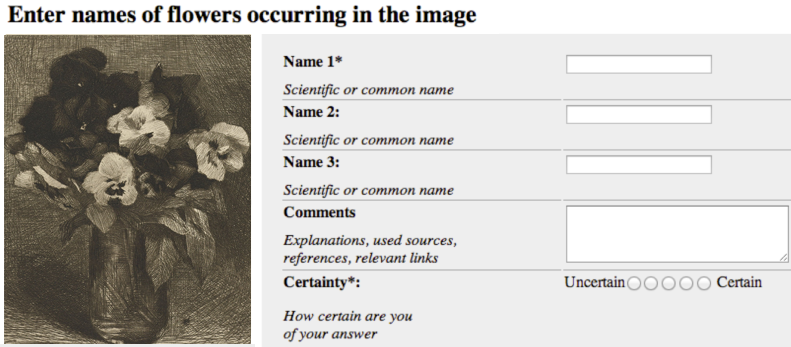
\includegraphics[height=3.65cm,natwidth=791,natheight=347]{ui.png}
\caption{User interface for annotation task.}
\label{fig:ui}
\end{figure}

\begin{table}
	\small
	\setlength{\tabcolsep}{2pt}
	\renewcommand{\arraystretch}{1.1}
	\begin{tabular}{| l | p{2cm} | p{2cm} |}
		\hline
		\textbf{\#}								& \textbf{Experts}	&\textbf{Crowd}	\\ \hline
		Annotators							& 4				& 75 (10 spam)		\\ \hline
		Annotation tasks performed				& 128			& 982 (214 spam)	\\ \hline
		Tags (excluding spam)					& 161			& 1077			\\ \hline
		Tags / annotation task					& 1: 105 (82\%)\newline
											2: 13 (10\%)\newline
											3: 10 (8\%)		& 1: 557 (73\%) \newline
															2: 113 (15\%) \newline
															3: 98 (12\%)
															\\ \hline
		Flower name tags						& 119	 		& 831			\\ \hline
		Confidence / annotation task				& $\mu$: 1.6 \newline
											$\rho$: 1.4 		& $\mu$: 2.5 \newline
															$\rho$: 1.3		\\ \hline
		Comments							& 31				& 306			\\ \hline
	\end{tabular}
	\caption{Overview of the experiment.}
	\label{tab:general}
\end{table}

\section{Results}
All 1238 tags were manually processed by 1) correcting spelling errors, 2) translating the tag into English, and 3) if the tag contained a flower name, identifying the corresponding taxonomy entry. 

Prints depicting a single flower, regardless of the flower prominence (SP and SNP), were almost always tagged by both experts and crowd workers with a single flower name. Prints of type MP were tagged with on average $1.8$ flower names by experts, and $1.7$ flower names by crowd workers. Prints of type MNP received a lower number of tags ($0.8$ and $1.0$ per task from experts and crowd workers respectively). In total 41\% of the experts flower tags, but only 20\% of the crowd worker tags, were the botanical name (instead of the common name).

Experts provided the tag ``unable'' in $33$ out of $128$ annotation tasks, related to $32$ distinct prints, with an average confidence value of $2.3$.  Crowd workers provided the tag ``unable'' in $85$ out of $768$ annotation tasks, related to $43$ distinct prints, with an average confidence value of $2.2$. For $21$ prints at least one expert and crowd worker indicated they were unable.

Experts provided the ``fantasy'' tag in $7$ out of $128$ annotation tasks, related to $7$ distinct prints, with an average confidence value of $2.4$. 
Crowd workers provided the ``fantasy'' tag in $53$ annotation tasks, related to $38$ distinct prints, with an average confidence value of $2.4$. For $3$ prints at least one expert and one crowd worker agreed on the presence of fantasy flowers.

For each tag provided for a print we calculated whether more than 50\% of the crowd annotators who annotated that print also provided that tag (majority voting). 
For 33 of these tags there was an agreement between crowd workers. However, these tags were all very common or frequently occurring flowers (e.g. rose, lily).

\section{Discussion and Conclusion}
We targeted crowd workers with unknown domain-specific knowledge. Despite this we found that they provide both botanical and common names for flowers. This suggests that crowdsourcing has the potential for providing useful annotations for knowledge intensive tasks, at a low cost.

Difficulty of annotation tasks clearly played a role in the tagging performance of the two groups which. This can be observed from the higher confidence for prints with prominent flowers and the low annotator agreement of crowd workers. Traditional algorithms such as majority voting are thus less useful for truth elicitation than in other image annotation tasks. Characteristics of these prints, prominence and amount of flowers, might make it more difficult to identify and name all the flowers in the print. This suggests the usage of a more articulated annotation process, where the recognition and identification of flowers are different annotation tasks, possibly to be assigned to different annotator groups. 

\vspace{5mm}

\noindent\textbf{Acknowledgements}
This publication was supported by the Dutch national program COMMIT. 

\bibliographystyle{abbrv}
\begin{thebibliography}{1}

\bibitem{Boer2012}
V.~Boer, M.~Hildebrand, L.~Aroyo, P.~Leenheer, C.~Dijkshoorn, B.~Tesfa, and
  G.~Schreiber.
\newblock Nichesourcing: Harnessing the power of crowds of experts.
\newblock In {\em Knowledge Engineering and Knowledge Management}, volume 7603
  of {\em LNCS}, pages 16--20. Springer, 2012.

\bibitem{Ellis2012}
A.~Ellis, D.~Gluckman, A.~Cooper, and A.~Greg.
\newblock Your paintings: A nation's oil paintings go online, tagged by the
  public.
\newblock {\em Museum and the Web}, 2012.

\bibitem{Gligorov2010}
R.~Gligorov, L.~B. Baltussen, J.~van Ossenbruggen, L.~Aroyo, M.~Brinkerink,
  J.~Oomen, and A.~van Ees.
\newblock Towards integration of end-user tags with professional annotations.
\newblock In {\em Proceedings of the WebSci10: Extending the Frontiers of
  Society On-Line}, 2010.

\bibitem{Trant2006}
J.~Trant, B.~Wyman, and Steve.
\newblock Investigating social tagging and folksonomy in art museums with
  steve.museum.
\newblock In {\em Proceedings of the WWW'06 Collaborative Web Tagging
  Workshop}, 2006.

\end{thebibliography}

\balancecolumns

\end{document}
